\begin{frame}[fragile]
\frametitle{pseudopilus: structure and function}
\begin{tabular}{m{.25\textwidth}|m{.75\textwidth}}
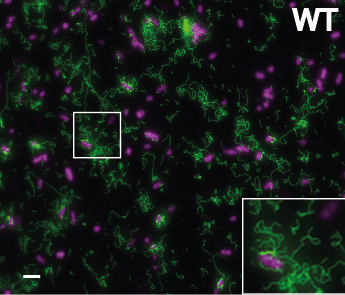
\includegraphics[width=.25\textwidth]{figures/pilusfluo.png}&
\includegraphics[width=.75\textwidth]{figures/pic_20130715_pilus.png}\cr
\end{tabular}
\begin{columns}
\begin{column}{.25\textwidth}
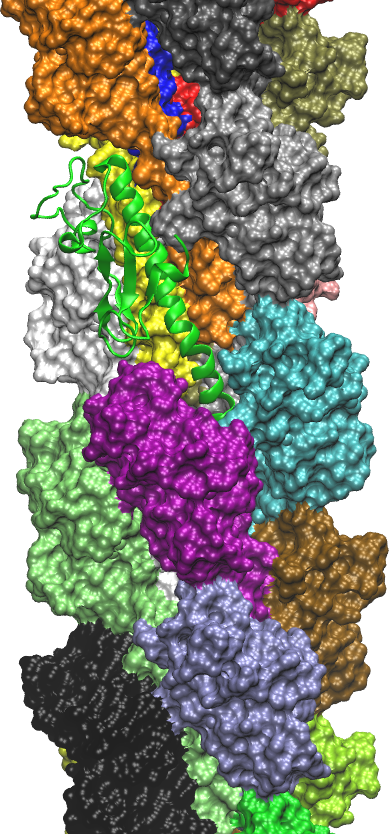
\includegraphics[width=\textwidth]{figures/20mer.png}
\end{column}
\begin{column}{.75\textwidth}
\begin{block}{Conformational sampling}
Pilus conformations generated by multi-stage minimization and molecular dynamic procedure in CNS using the CHARMM PARAM19 force field ...
\end{block}
\footnotesize{From Campos et al. 2010}
\end{column}
\end{columns}
\end{frame}
